\documentclass{article}

% packages for highlighting
\usepackage{xcolor}
\usepackage{soul}

% packages for annotation
\usepackage{todonotes}

% packages for indentation
\usepackage{indentfirst}

% packages for tables
\usepackage{booktabs}
\usepackage{multirow}
\usepackage{tablefootnote}

% packages for bibliography
\usepackage[style=apa,backend=biber,doi=false,isbn=false,url=false,eprint=false]{biblatex}
\addbibresource{../../.resources/My Library.bib}

% packages for flowchart
\usepackage{tikz}
\usetikzlibrary{positioning}
\usetikzlibrary{calc}

% document information
\title{Effects of Music on Verbal Memory}
\author{some author}

\begin{document}

\maketitle{}

\section{Introduction}

We are capable of memorizing a lot of things without effort right from infancy. Yet we never really know how we managed to do that. Especially, the lack of understanding about memory lead us to suffer when we failed to recall what we should have memorized, say, when we are taking a test and having trouble recalling the right answer. 

In this paper, I first summarize the current researches on the common factors that affect memory. Then I \hl{  }. I close this paper by \hl{  }. I wish to show that \hl{  }.

\section{Literature Review}

How can we know about the factors that would affect memory? Intuitively, we can conduct a simple experiment in the following manner. If some factor \textit{A} makes people's memory better (or worse) than the people in control group, and \textit{A} is not present in control group, then we may conclude that this \textit{A} has an impact on human memory. However, conclusions derived from this manner is severely weakened by the fact that individual difference is so big that it is very hard to control variables that may affect the conclusion. Therefore, we must pursuit a more biologically plausible way.

The rough idea is that, as long as we understand the physical mechanism of human memory, and some factor \textit{A} can enhance (or suppress) this mechanism, then we would happily conclude that \textit{A} has an impact on our memory. Of course, the mechanism of human memory is still not entirely clear today owing to the complexity of human brain. However, developing the understanding of such mechanism is beyond the scope of this paper, and this paper would \hl{mostly?} take the current prevailing view on this mechanism for granted.

\subsection{The mechanism and Related Structures}

Though sharing the same word, memory in fact has several different kinds. Intuitively, memory is what we recollect consciously, i.e.\ how to prove Pythagorean theorem. But some memories are also subconscious. For instance, nothing really pops up in our mind when we begin to ride a bike. We just somehow control it. This indicates that some memory is at work, but not at the conscious level. In psychology, this kind of subconscious memory is called \textit{implicit memory}, as opposed to the conscious one called \textit{explicit memory}.\footnote{Some scholars also use the ``declarative-nondeclarative'' dichotomy, (see~\cite{michaelianMemory2017}). As applied to human, there is little difference between the ``declarative-nondeclarative'' and ``explicit-implicit'' taxonomy \autocite[p.480]{kolbIntroductionBrainBehavior2019}.} In addition, \textit{Emotion memory} has both conscious and subconscious character. For instance, someone would reexperience the joy when consciously describing a past event, which shows the explicit nature of emotional memory. Implicit character, on the other hand, is illustrated by conditioning, i.e. conditioned fear (for an explanation of conditioned fear, see~\cite[p.478]{kolbIntroductionBrainBehavior2019}). 

Though still under dispute, the overall consensus on the anatomy of explicit memory is reached around the 1990s \autocite[p. 487]{kolbIntroductionBrainBehavior2019}. The brain sections involved in explicit memory are mainly around the medial temporal region, the prefrontal cortex and the related structures. As the figure~\ref{MechofExpMem} illustrates, sensory data are passed from sensory cortices to perirhinal and parahippocampal cortex. Then entorhinal cortex integrates these data and further send them to hippocampus. This connection also goes backwards, which may explain why we are able to retrieve it consciously. 

\begin{figure}[h]
    \centering
    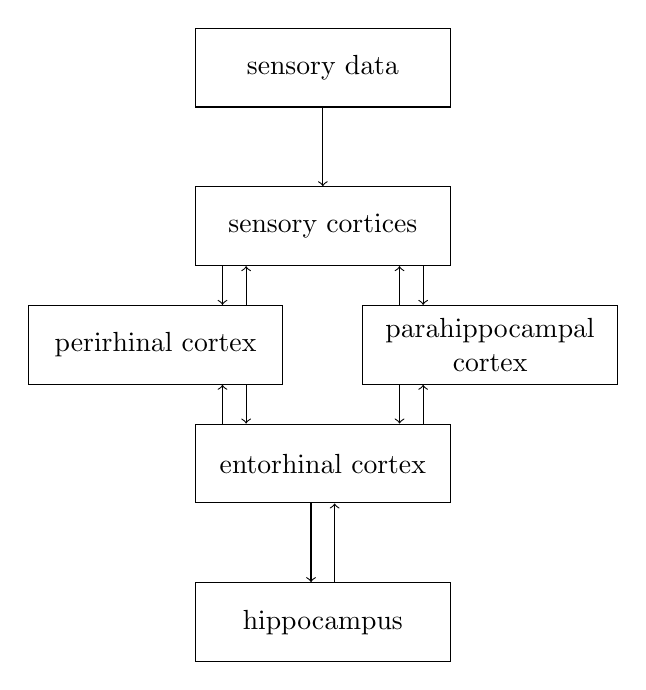
\begin{tikzpicture}[
        box/.style={rectangle, draw=black, text width=3cm, minimum height=1cm, align=center}
    ]
    
    \node[box] (2_1) {perirhinal cortex};
    \node[box] (2_2) [right=of 2_1] {parahippocampal cortex};
    \coordinate (COL2_MID) at ($(2_1)!0.5!(2_2)$);
    \node[box] (1_1) [above=of COL2_MID]{sensory cortices};
    \node[box] (0_1) [above=of 1_1]{sensory data};
    \node[box] (3_1) [below=of COL2_MID] {entorhinal cortex};
    \node[box] (4_1) [below=of 3_1] {hippocampus};

    \draw[->] (0_1.south) to (1_1.north);
    
    \draw[->] ([xshift=0.35cm]1_1.south west) to ([xshift=0.35cm]1_1.south west |- 2_1.north);
    \draw[<-] ([xshift=0.65cm]1_1.south west) to ([xshift=0.65cm]1_1.south west |- 2_1.north);

    \draw[->] ([xshift=-0.35cm]1_1.south east) to ([xshift=-0.35cm]1_1.south east |- 2_2.north);
    \draw[<-] ([xshift=-0.65cm]1_1.south east) to ([xshift=-0.65cm]1_1.south east |- 2_2.north);

    \draw[->] ([xshift=0.35cm]3_1.north west) to ([xshift=0.35cm]3_1.north west |- 2_1.south);
    \draw[<-] ([xshift=0.65cm]3_1.north west) to ([xshift=0.65cm]3_1.north west |- 2_1.south);

    \draw[->] ([xshift=-0.35cm]3_1.north east) to ([xshift=-0.35cm]3_1.north east |- 2_2.south);
    \draw[<-] ([xshift=-0.65cm]3_1.north east) to ([xshift=-0.65cm]3_1.north east |- 2_2.south);

    \draw[->] ([xshift=-0.15cm]3_1.south) to ([xshift=-0.15cm]4_1.north);
    \draw[<-] ([xshift=0.15cm]3_1.south) to ([xshift=0.15cm]4_1.north);
    \end{tikzpicture}
    \caption{Mechanism of Explicit Memory\protect\footnotemark}
    \label{MechofExpMem}
\end{figure}
\footnotetext{Reproduced from~\cite[p. 487]{kolbIntroductionBrainBehavior2019}, Figure 14-9, slightly modified}

Implicit memory, on the other hand, is more complicated and controversial (for details, see~\cite{reberNeuralBasisImplicit2013}). However, generally speaking, critical areas for implicit learning includes motor cortex and surrounding areas, striatum and associated basal ganglia structures as well as the cerebellum \autocite[p. 470]{eichenbaumConditioningConsciousRecollection2001}. \textcite{kolbIntroductionBrainBehavior2019} also proposed a hypothesized circuit, reproduced as Figure~\ref{MechofImplMem}. The center of this path, basal ganglia, receive information from both the entire neocortex and and cells in the substantia nigra. Basal ganglia in turn project these data to ventral thalamus and then to premotor cortex. This circuit is unidirectional, which may explain why consciousness is not involved in this process. 

\begin{figure}[h]
\centering
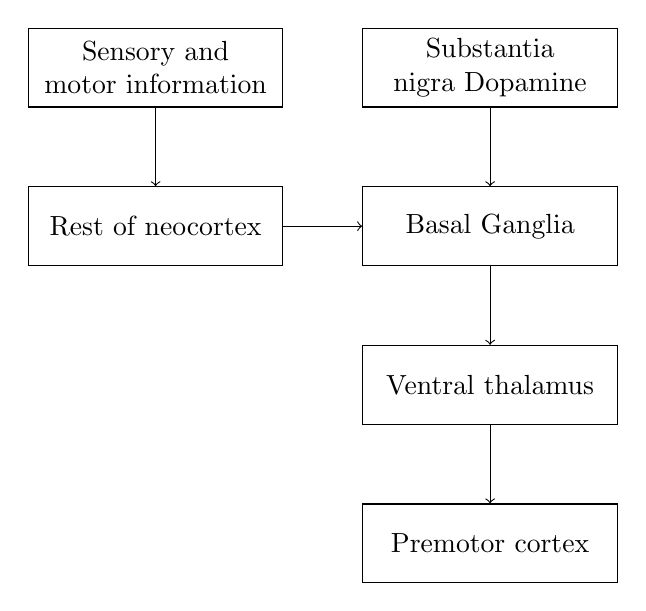
\begin{tikzpicture}[
    box/.style={rectangle, draw=black, text width=3cm, minimum height=1cm, align=center}
]
\node[box] (1_1) {Sensory and motor information};
\node[box] (1_2) [right=of 1_1] {Substantia nigra Dopamine};
\node[box] (2_1) [below=of 1_1] {Rest of neocortex};
\node[box] (2_2) [below=of 1_2] {Basal Ganglia};
\node[box] (3_2) [below=of 2_2] {Ventral thalamus};
\node[box] (4_2) [below=of 3_2] {Premotor cortex};

\draw[->] (1_1.south) to (2_1.north);
\draw[->] (1_2.south) to (2_2.north);
\draw[->] (2_1.east) to (2_2.west);
\draw[->] (2_2.south) to (3_2.north);
\draw[->] (3_2.south) to (4_2.north);
\end{tikzpicture}

\caption{Proposed Mechanism of Explicit Memory\protect\footnotemark}
\label{MechofImplMem}    
\end{figure}
\footnotetext{Reproduced from~\cite[p.494]{kolbIntroductionBrainBehavior2019}, Figure 14-15B without modification except styles}

As for emotional memory, both explicit circuit and implicit circuit are involved. Amygdala, however, plays an unique role in its mechanism \autocite{davisRoleAmygdalaFear}. People with amygdala malfunction show no emotional memory while having both explicit and implicit memory intact \autocite[p.494]{kolbIntroductionBrainBehavior2019}. \textcite[p.494]{kolbIntroductionBrainBehavior2019} also provide us with a simplified diagram, displayed as Figure~\ref{MechofEmoMem}.

\begin{figure}[h]
\centering

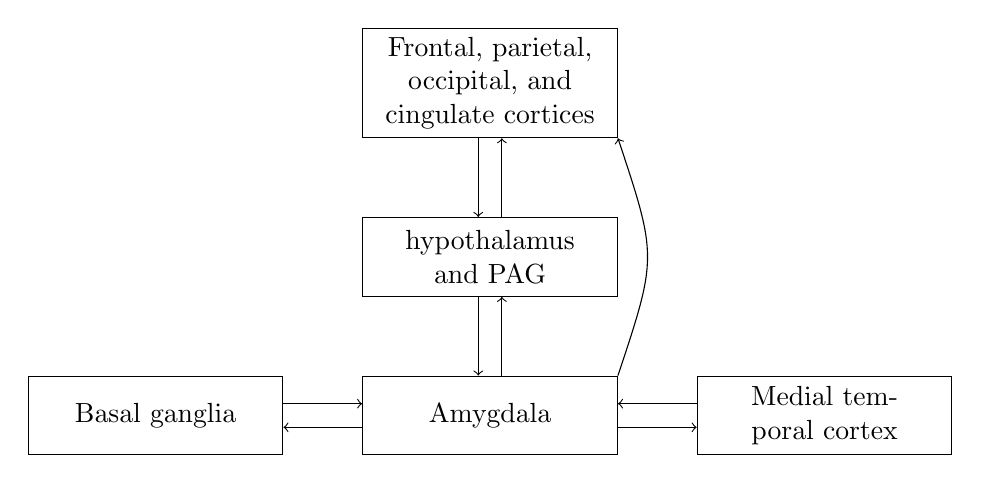
\begin{tikzpicture}[
    box/.style={rectangle, draw=black, text width=3cm, minimum height=1cm, align=center}
]
\node[box] (1_2) {Frontal, parietal, occipital, and cingulate cortices};
\node[box] (2_2) [below=of 1_2] {hypothalamus and PAG};
\node[box] (3_2) [below=of 2_2] {Amygdala};
\node[box] (3_1) [left=of 3_2] {Basal ganglia};
\node[box] (3_3) [right=of 3_2] {Medial temporal cortex};

\draw[->] ([xshift=-0.15cm]1_2.south) to ([xshift=-0.15cm]2_2.north);
\draw[<-] ([xshift=0.15cm]1_2.south) to ([xshift=0.15cm]2_2.north);

\draw[->] ([xshift=-0.15cm]2_2.south) to ([xshift=-0.15cm]3_2.north);
\draw[<-] ([xshift=0.15cm]2_2.south) to ([xshift=0.15cm]3_2.north);
\draw[<-] (1_2.south east) .. controls ([xshift=0.5cm]2_2.east) .. (3_2.north east);

\draw[->] ([yshift=0.15cm]3_1.east) to ([yshift=0.15cm]3_2.west);
\draw[<-] ([yshift=-0.15cm]3_1.east) to ([yshift=-0.15cm]3_2.west);

\draw[->] ([yshift=0.15cm]3_3.west) to ([yshift=0.15cm]3_2.east);
\draw[<-] ([yshift=-0.15cm]3_3.west) to ([yshift=-0.15cm]3_2.east);

\end{tikzpicture}
\caption{Mechanism of Explicit Memory\protect\footnotemark}
\label{MechofEmoMem}
\end{figure}
\footnotetext{Reproduced from~\cite[p.494]{kolbIntroductionBrainBehavior2019}, Figure 14-15B, slightly modified}

Another popular model, proposed by \textcite{atkinsonHumanMemoryProposed1968}, distinguishes memory by the temporal duration. Ultra short-term storage is formed in the process of sensory registration, which lasts less than one second. Short-term storage lives up to thirty seconds. Long-term storage refers to memory that lasts indefinitely long period of time. This classification adds the prefrontal cortex to our attention, for it plays a critical role in short-term memory \autocite[p. 472]{eichenbaumConditioningConsciousRecollection2001}.

Though the details are still enigmatic, the general mechanism of memory is now clear. This instantly follows that once the corresponding brain structure goes wrong, the related memory functions will also be compromised.

\subsection{Common Factors}

The first thing that directly comes to our mind that would harm the brain would probably be chemicals. For instance, when people are under stress, adrenal cortex releases \textit{glucocorticoids} due to our fight-or-flight response. This activates our amygdala and enhance our memory on the stress-related events \autocite{sapolskyStressAgingBrain1992}. Worse, evidence has shown that glucocorticoids would temporarily block memory retrieval \autocite[pp.119-144]{roozendaalStressMemoryAmygdala2009}, and long-term exposure to glucocorticoids kills hippocampal cells, which plays a critical role in explicit memory \autocite{sapolskyStressAgingBrain1992}. 

Alcohol is another chemical that is detrimental to memory. It suppresses the activity of pyramidal cells, the cells mainly found in medial temporal cortex, and impairs the formation of Hippocampal LTP\footnote{Long-Term Potentiation (LTP) mechanism, discovered by \textcite{blissLonglastingPotentiationSynaptic1973}, is considered as the mechanism of how brain learns new things}. Long-term alcoholism causes thiamine deficiency, which results the death of brain cells including medial regions of the thalamus and the mammillary bodies of the hypothalamus \autocite{martinRoleThiamineDeficiency2003}. This is known as \textit{Korsakoff Syndrome}. 

Iron deficiency can also affect memory given that iron participates in the metabolic of hippocampal cells. The deficiency of iron will cause abnormal hippocampal structure and plasticity in adults. Early life iron deficiency, on the other hand, impairs hippocampal development which in turn causes cognitive functions \autocite{frethamRoleIronLearning2011}.

Apart from chemicals, age is also an important factor, since old people tends to suffer from Alzheimer Disease and have slippery memory. This is usually caused by neuritic plaques, concentrated especially in temporal lobe areas related to memory \autocite{kolbIntroductionBrainBehavior2019}. In addition, older adults shows different patterns of brain activation from younger adults during explicit and implicit encoding and retrieval tasks \autocite{backmanBrainActivationYoung1997}.

Sleep also enhance memory the the process called \textit{consolidation}. Research has shown that both SWS and REM contributes to solidifying knowledge learnt in day \autocite{diekelmannMemoryFunctionSleep2010}.

\printbibliography{}
\end{document}